\documentclass[12pt]{article}

%%%%%%%%%%%%%%%%%%%%%%%%%%%%%%%%%%%%%%%%%%%%%%%%%%%%%%%%%%%%%%%%%%%%%%%%%%%%%%%%%%%%%%
%%%%%%%%%%%%%%%%%%% PREAMBLE (Optimized Version) %%%%%%%%%%%%%%%%%%%
% --- Language and Encoding ---
\usepackage[utf8]{inputenc}
\usepackage[T1]{fontenc}

% --- Math Packages ---
\usepackage{amsfonts, amsmath, amssymb} 

% --- Fonts ---
\usepackage{libertine} 
\usepackage{mathpazo} 

% --- Layout and Graphics ---
\usepackage{fullpage}
\usepackage{graphicx} 
\usepackage{booktabs} 
\usepackage{float}
\usepackage{subcaption}

% --- Algorithms ---
\usepackage{algorithm}
\usepackage{algpseudocode}

% --- Bibliography (Updated for APA via BibLaTeX) ---
\usepackage[style=apa, backend=biber]{biblatex}
\addbibresource{references.bib}

% --- Hyperlinks (Should be loaded last in most cases) ---
\usepackage{hyperref}
\hypersetup{
    colorlinks = true,
    linkcolor = blue,
    urlcolor  = blue,
    citecolor = blue,
    anchorcolor = blue
}
\urlstyle{same}
%%%%%%%%%%%%%%%%%%%%%%%%%%%%%%%%%%%%%%%%%%%%%%%%%%%%%%%%%%%%%%%%%%%%%%%%%%%%%%%%%%%%%%

\begin{document}

\title{Simulation-Based Inference for an Adaptive-Network Epidemic Model}
\date{\today}
\maketitle
\thispagestyle{empty}

\centerline{\textbf{Group Composition:} Yohei Kiguchi (A0308628X, e1399068@u.nus.edu)}
\vspace{1em}
\hrule
\vspace{1.5em}

% === MAIN CONTENT ===
\section{Introduction}
Infectious disease dynamics are heavily influenced by the underlying contact network of individuals.
In standard epidemic models, the network structure is often assumed to be static.
However, real-world populations exhibit adaptive behavior where individuals modify their contacts in response to the epidemic.
This project investigates a Susceptible-Infected-Recovered (SIR) model on an adaptive network, where susceptible individuals break links with infected neighbors and form new connections to non-infected agents.
The feedback loop between the disease spread and the evolving network topology makes the likelihood function for this model intractable \parencite{demirel2017dynamics}.
Standard statistical methods, such as Maximum Likelihood Estimation, are therefore difficult to apply directly to such complex stochastic systems.
To address this challenge, we employ Simulation-Based Inference (SBI) to estimate the core parameters: the infection probability $\beta$, the recovery probability $\gamma$, and the rewiring probability $\rho$.
Since SBI requires a significant number of forward simulations, we implemented a high-performance simulator using Python and Numba to ensure computational efficiency during the inference process.
We are provided with observed data from $R=40$ independent realizations of the stochastic process.
The available measurements include time-series data for the infected fraction and rewiring counts, as well as final degree histograms at the conclusion of the simulation.
The goal of this report is to describe the implementation of Approximate Bayesian Computation (ABC) and explore advanced sequential methods to obtain robust posterior distributions for the unknown parameters.
% Section 02: ABC Rejection
% Section 02: ABC Rejection
\section{Approximate Bayesian Computation: Rejection Sampling}

As a baseline for our inference task, we first implemented the standard Approximate Bayesian Computation (ABC) rejection algorithm \parencite{beaumont2002approximate}.
In this framework, a candidate parameter vector $\theta = (\beta, \gamma, \rho)$ is sampled directly from the joint prior distribution.
For each sampled $\theta$, the adaptive-network SIR simulator is executed to generate a synthetic realization of the epidemic.
The candidate $\theta$ is accepted if the distance between the summary statistics of the simulated and observed data falls below a tolerance threshold $\epsilon$.

For this baseline analysis, we utilized a 4-dimensional summary statistic vector: peak infection fraction, total rewiring events, final degree variance, and time to peak infection.
To ensure each statistic contributes equally to the distance metric, the Euclidean distance is calculated after normalizing these features using the standard deviations obtained from independent replicates.
The detailed theoretical justification for selecting these specific statistics over simpler metrics is discussed in Section 3.

In our experiments, we performed $N=100,000$ forward simulations using the optimized Numba-based simulator.
Setting the normalized Euclidean distance tolerance to $\epsilon = 4.0$, the algorithm accepted 5,343 particles, resulting in an acceptance rate of approximately 5.3\%.
The execution required approximately 177 seconds on a standard compute node.

\begin{figure}[H]
    \centering
    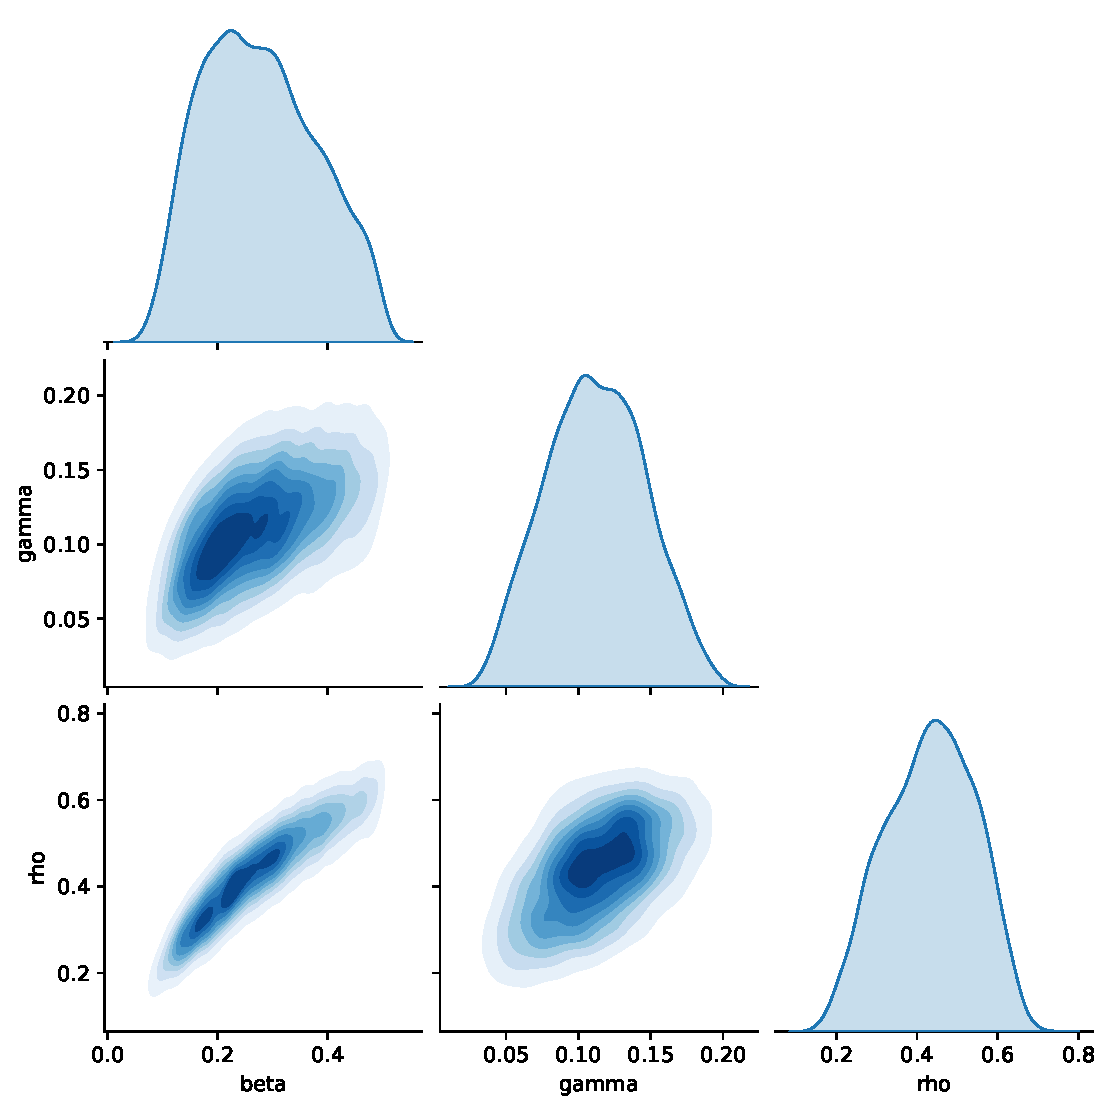
\includegraphics[width=0.6\textwidth]{plots/posterior_pairplot_s4_time.pdf}
    \caption{Pairwise posterior distributions obtained via Baseline ABC Rejection Sampling ($\epsilon=4.0$).}
    \label{fig:abc_rejection_pairplot}
\end{figure}

The resulting pairwise plots (Figure \ref{fig:abc_rejection_pairplot}) indicate that the posterior probability mass begins to localize within the parameter space, partially resolving the equifinality between $\beta$ and $\rho$.
However, the computational bottleneck caused by the curse of dimensionality restricted the number of accepted samples given a feasible time constraint \parencite{nott2014approximate}.
Consequently, the approximated posterior distribution remained relatively noisy and insufficiently dense for robust inference.
These results clearly demonstrate that naive rejection sampling is computationally inefficient for our parameter space, strongly motivating the transition to advanced sequential Monte Carlo methods.
\section{Summary Statistics}

In Simulation-Based Inference (SBI), the choice of summary statistics $S(y)$ is critical as it determines the amount of information extracted from high-dimensional raw data \parencite{beaumont2002approximate}.
In this section, we describe the systematic process used to identify a set of informative features that resolve parameter non-identifiability.

\subsection{The Identification Challenge: The $\beta$-$\rho$ Trade-off}

Initial experiments using basic summary statistics revealed a significant "ridge" in the joint posterior distribution of the infection rate $\beta$ and the rewiring rate $\rho$.
This ridge suggests an equifinality problem where a high-infection/high-rewiring scenario and a low-infection/low-rewiring scenario produce similar overall infection scales.
The model struggles to distinguish between a virus that spreads rapidly but is countered by fast network adaptation, and a virus that spreads slowly in a more stable network \parencite{demirel2017dynamics}.
To resolve this, we performed a comparative simulation analysis between parameter sets at both ends of the observed ridge.
Figure \ref{fig:sir_comparison} illustrates the distinct temporal dynamics of these cases, suggesting that peak timing and structural network changes are key to decoupling these parameters.

\begin{figure}[H]
    \centering
    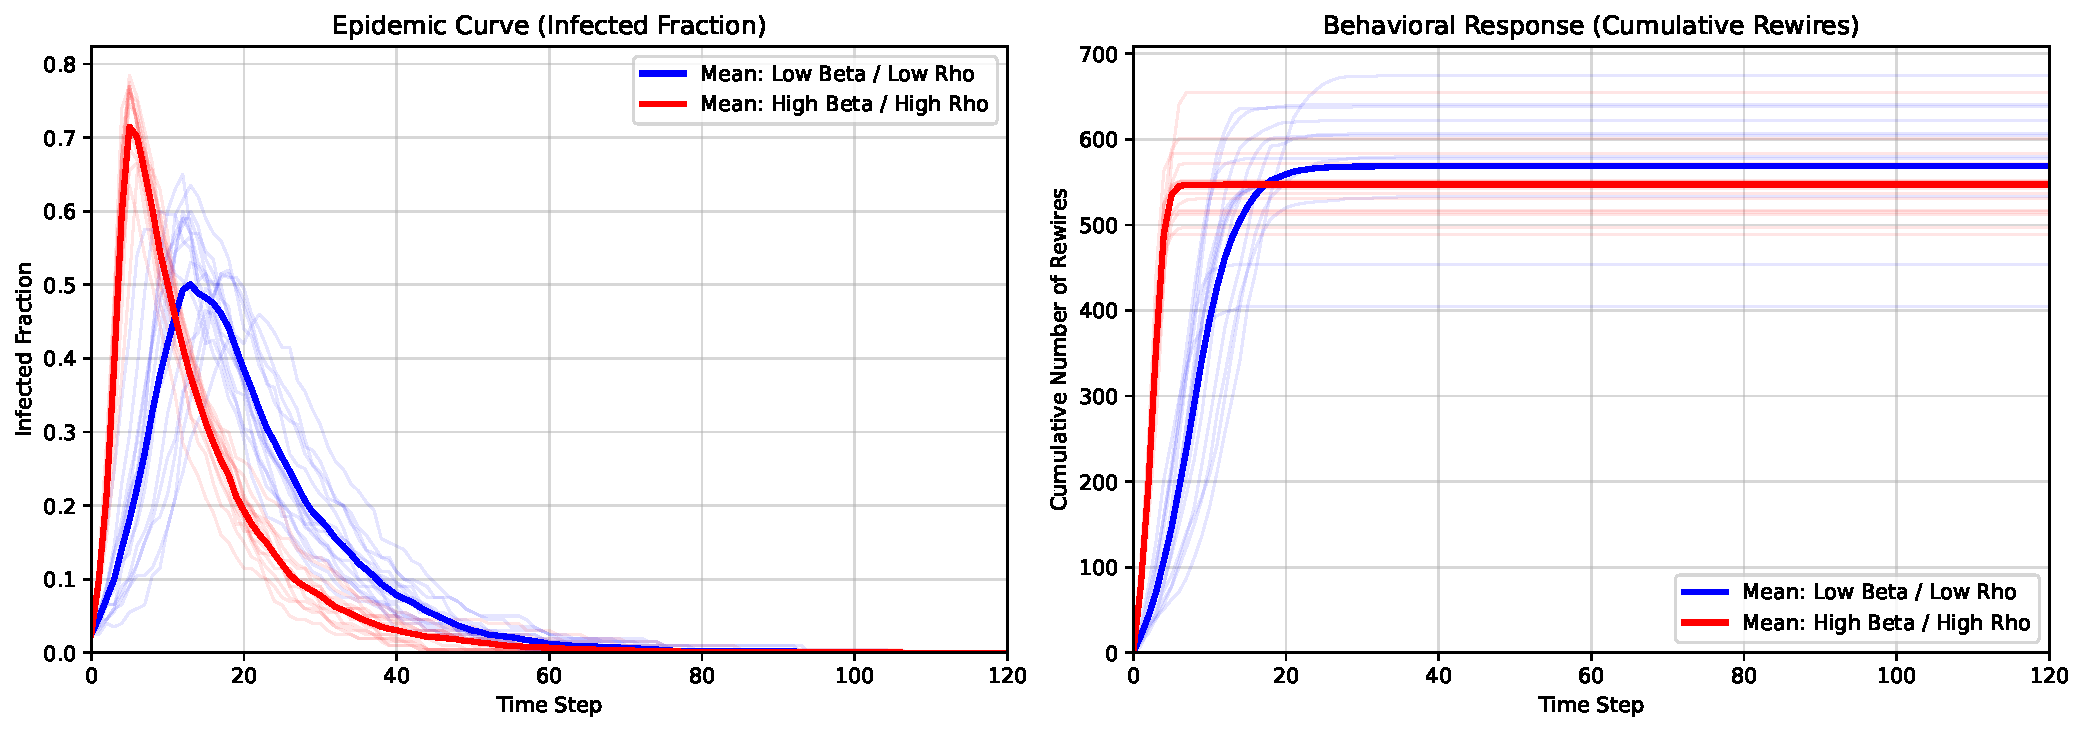
\includegraphics[width=0.9\textwidth]{plots/smc_abc_SIR_plot_1.pdf}
    \caption{Comparison of SIR dynamics and rewiring behavior for High $\beta$/High $\rho$ versus Low $\beta$/Low $\rho$ scenarios.}
    \label{fig:sir_comparison}
\end{figure}

\subsection{Selection of Informative Features}

Based on the observed dynamics, we expanded our summary statistic vector to five dimensions to capture both temporal and topological information:

\begin{itemize}
    \item \textbf{$s_1$: Peak Infected Fraction}: Captures the maximum intensity of the outbreak.
    \item \textbf{$s_2$: Log Rewire-to-Infection Ratio}: Measures the efficiency of behavioral response relative to the total infection risk.
    \[ s_2 = \log \left( \frac{\sum_{t} R_t}{\sum_{t} I_t + \epsilon_{small}} \right) \]
    \item \textbf{$s_3$: Log Final Degree Variance}: Detects the topological "scars" left by the rewiring process on the network structure.
    \item \textbf{$s_4$: Log Weighted Infection Timing}: Captures the "center of mass" of the epidemic curve, providing a robust metric for peak timing.
    \[ s_4 = \log \left( \frac{\sum_{t} t \cdot I_t}{\sum_{t} I_t} \right) \]
    \item \textbf{$s_5$: Log Maximum Step Rewire Rate}: Captures the burstiness of the behavioral response.
\end{itemize}

While these statistics are highly informative, they exhibit significant internal correlations.
A naive Euclidean distance fails to account for this dependent structure, which necessitates the use of a more sophisticated distance metric.
The implementation of the Mahalanobis distance to address these correlations is detailed in Section 4.2.

% \subsection{Distance Metric: Mahalanobis Distance}

% Because these statistics are inherently correlated (e.g., peak height and timing), a naive Euclidean distance is suboptimal. 
% In our final SMC-ABC implementation, we employ the Mahalanobis distance:
% \begin{equation}
%     d(s, s_{obs}) = \sqrt{(s - s_{obs})^T \mathbf{\Sigma}^{-1} (s - s_{obs})}
% \end{equation}
% where $\mathbf{\Sigma}$ is the covariance matrix estimated from the observed replicates. 
% This approach decorrelates the summary statistics and ensures that the inference process is sensitive to the unique information provided by each feature, effectively breaking the $\beta$-$\rho$ ridge.
% Section 04: Advanced Sequential Monte Carlo Methods
\section{Advanced Sequential Monte Carlo Methods}

The naive rejection sampling discussed in Section 2 is computationally prohibitive for complex models with high-dimensional summary statistics.
To ensure robust inference, we implemented a Sequential Monte Carlo (SMC) ABC algorithm, which iteratively refines the posterior approximation.

\subsection{SMC-ABC: Efficiency and Adaptive Sampling}

The primary advantage of SMC-ABC is its adaptive sampling efficiency.
Unlike rejection sampling, which suffers from low acceptance rates as the tolerance $\epsilon$ decreases, SMC-ABC maintains a population of $M$ particles that are evolved through a sequence of intermediate distributions \parencite{beaumont2009adaptive, moores2015preprocessing}.
By using an adaptive tolerance schedule—where $\epsilon_t$ is determined by the $\alpha$-th percentile of the previous generation's distances—the algorithm guarantees that we obtain a pre-specified number of samples even at very small tolerances.
The general structure of our implementation is detailed in Algorithm \ref{alg:smc_abc}.

\begin{algorithm}[H]
\caption{Sequential Monte Carlo ABC with Adaptive Tolerance}
\label{alg:smc_abc}
\begin{algorithmic}[1]
    \Require Observed summaries $s_{obs}$, Prior $\pi(\theta)$, Number of particles $M$, Target tolerance $\epsilon_T$
    \Ensure Weighted particles $\{(\theta_i^{(T)}, w_i^{(T)})\}_{i=1}^M$
    
    \State \textbf{Initialization:} Sample $M$ particles $\{\theta_i^{(0)}\}$ from $\pi(\theta)$ and set weights $w_i = 1/M$.
    \For{generation $t = 1$ \textbf{to} $T$}
        \State Set $\epsilon_t$ as the $\alpha$-th percentile of distances from generation $t-1$.
        \State Compute covariance $\Sigma_{t-1}$ of the current population for the perturbation kernel.
        \While{accepted particles $< M$}
            \State Sample $\theta^*$ from $\{\theta_k^{(t-1)}\}$ with weights $w_k^{(t-1)}$.
            \State Perturb $\theta^{**} \sim \mathcal{N}(\theta^*, \Sigma_{t-1})$ using a multivariate normal kernel.
            \State Simulate $y^{**} \sim f(y|\theta^{**})$ and compute $s^{**} = S(y^{**})$.
            \If{$d(s^{**}, s_{obs}) \le \epsilon_t$}
                \State Store $\theta^{**}$ and calculate importance weight $w^{**}$.
            \EndIf
        \EndWhile
        \State Normalize weights $w_i^{(t)}$.
    \EndFor
\end{algorithmic}
\end{algorithm}

\subsection{Comparison of Distance Metrics: Euclidean vs. Mahalanobis}

In our baseline SMC implementation (weighted Euclidean distance), the posterior for $\beta$ and $\rho$ exhibited a strong "ridge," indicating the model's struggle to decouple the two parameters.
By transitioning to the Mahalanobis distance, we accounted for the covariance structure $\mathbf{\Sigma}$ of the 5D summary statistics \parencite{nott2014approximate}:
\begin{equation}
    d(s, s_{obs}) = \sqrt{(s - s_{obs})^T \mathbf{\Sigma}^{-1} (s - s_{obs})}
\end{equation}
As shown in Figure \ref{fig:dist_comparison}, the Mahalanobis metric (b) noticeably reduces the artificial correlation in the posterior compared to the standard approach (a), allowing for a more localized and accurate identification of the true parameter values.

\begin{figure}[H]
    \centering
    \begin{subfigure}[b]{0.48\textwidth}
        \centering
        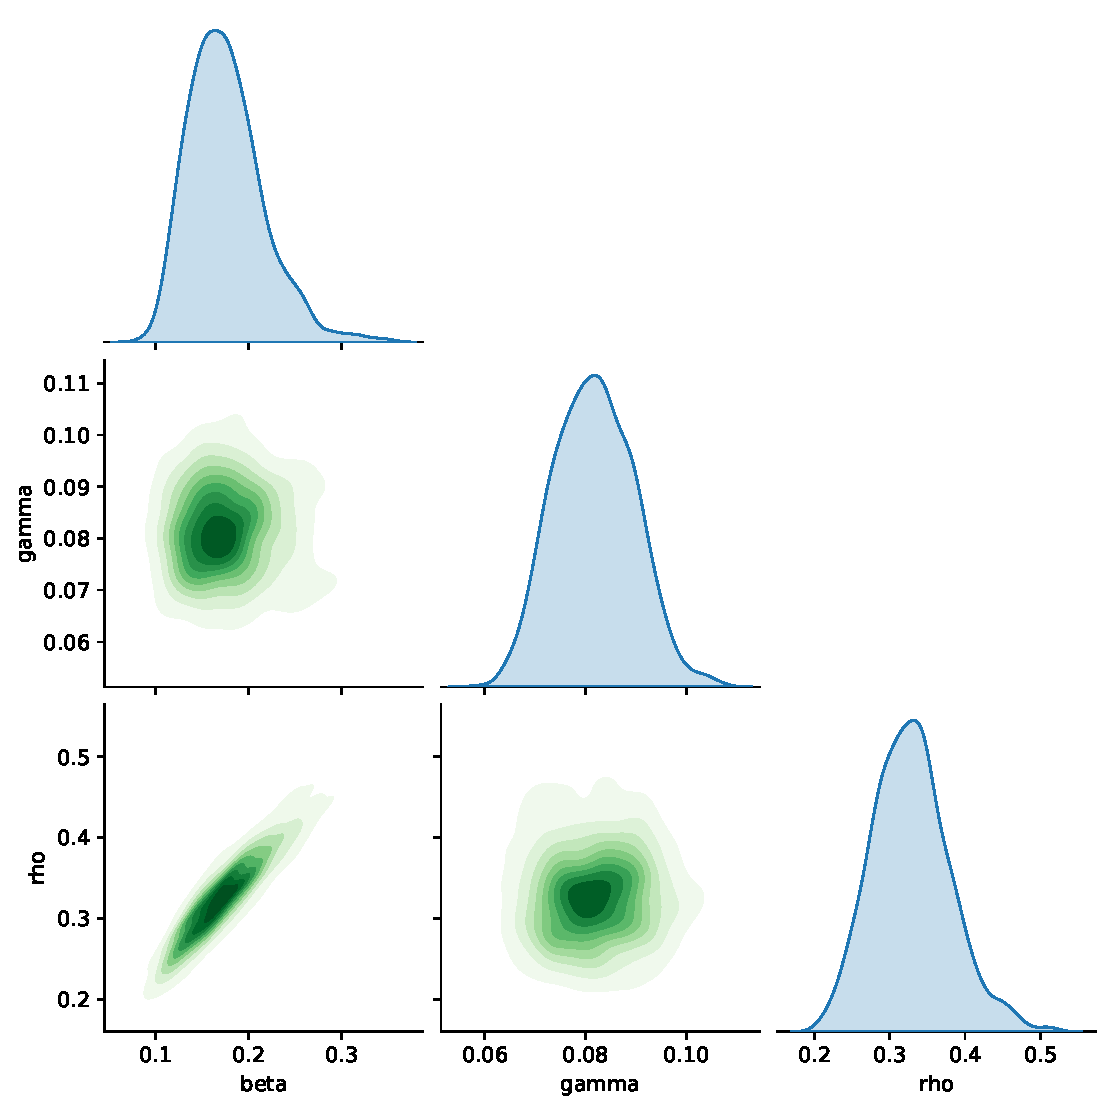
\includegraphics[width=\textwidth]{plots/smc_abc_pairplot_s4_weighted_time.pdf}
        \caption{Weighted Euclidean (Baseline)}
        \label{fig:dist_euclidean}
    \end{subfigure}
    \hfill
    \begin{subfigure}[b]{0.48\textwidth}
        \centering
        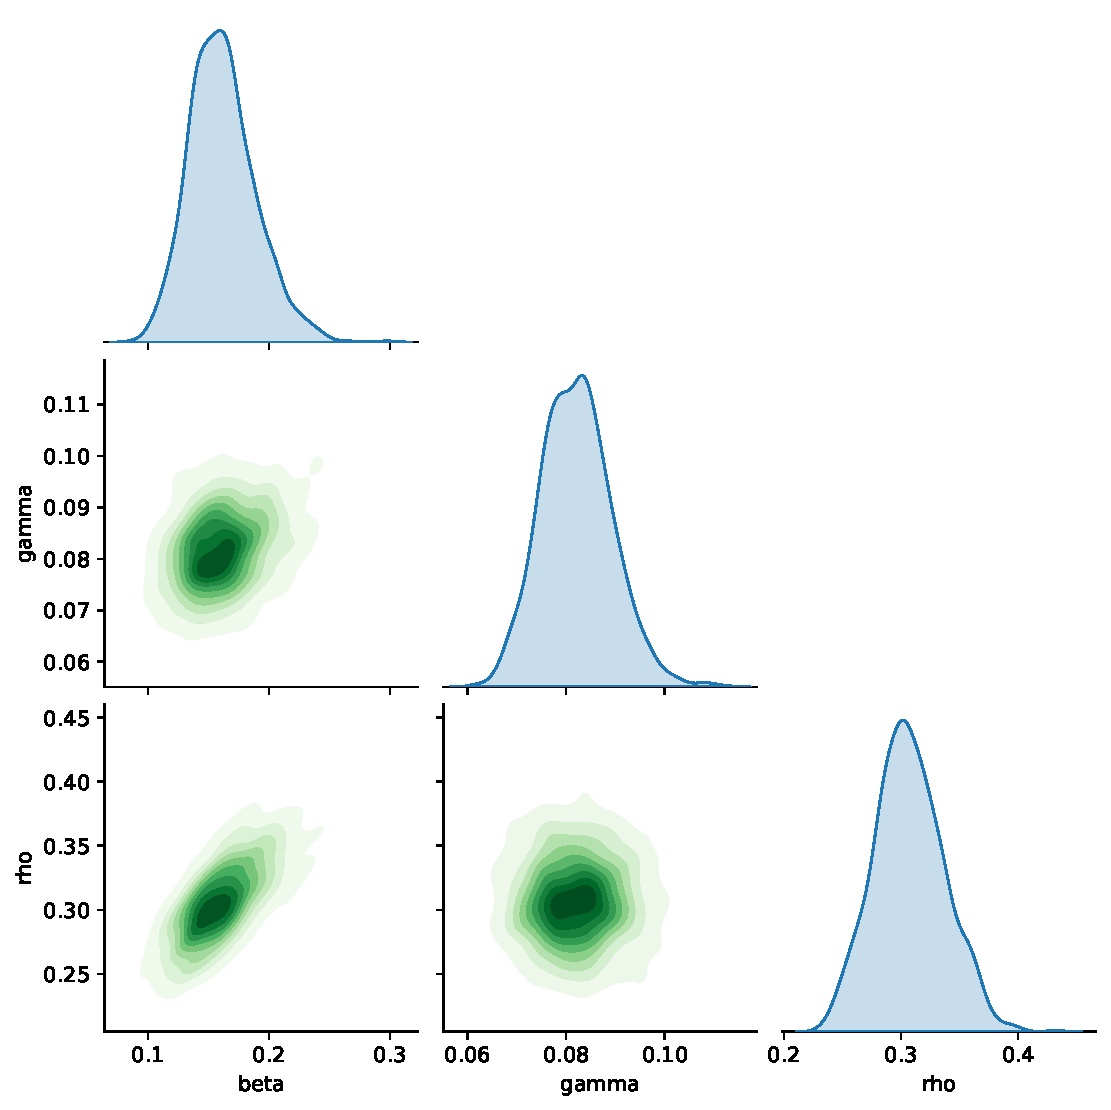
\includegraphics[width=\textwidth]{plots/smc_abc_pairplot_s5_mahalanobis.pdf}
        \caption{Mahalanobis Distance}
        \label{fig:dist_mahalanobis}
    \end{subfigure}
    \caption{Posterior comparison between distance metrics.
The Mahalanobis metric effectively decorrelates the summary statistics, breaking the $\beta$-$\rho$ trade-off ridge.}
    \label{fig:dist_comparison}
\end{figure}

\subsection{Post-processing: Local Linear Regression Adjustment}

To further refine the results and neutralize the bias introduced by a non-zero $\epsilon$, we applied a local linear regression adjustment \parencite{beaumont2002approximate}.
Figure \ref{fig:reg_comparison} illustrates the dramatic "sharpening" effect: the marginal distributions become significantly tighter and more centered around the true values \parencite{blum2017regression}.
Quantitative improvements are summarized in Table \ref{tab:regression_improvement}, showing an average precision gain of approximately 30\%.

\begin{figure}[H]
    \centering
    \begin{subfigure}[b]{0.48\textwidth}
        \centering
        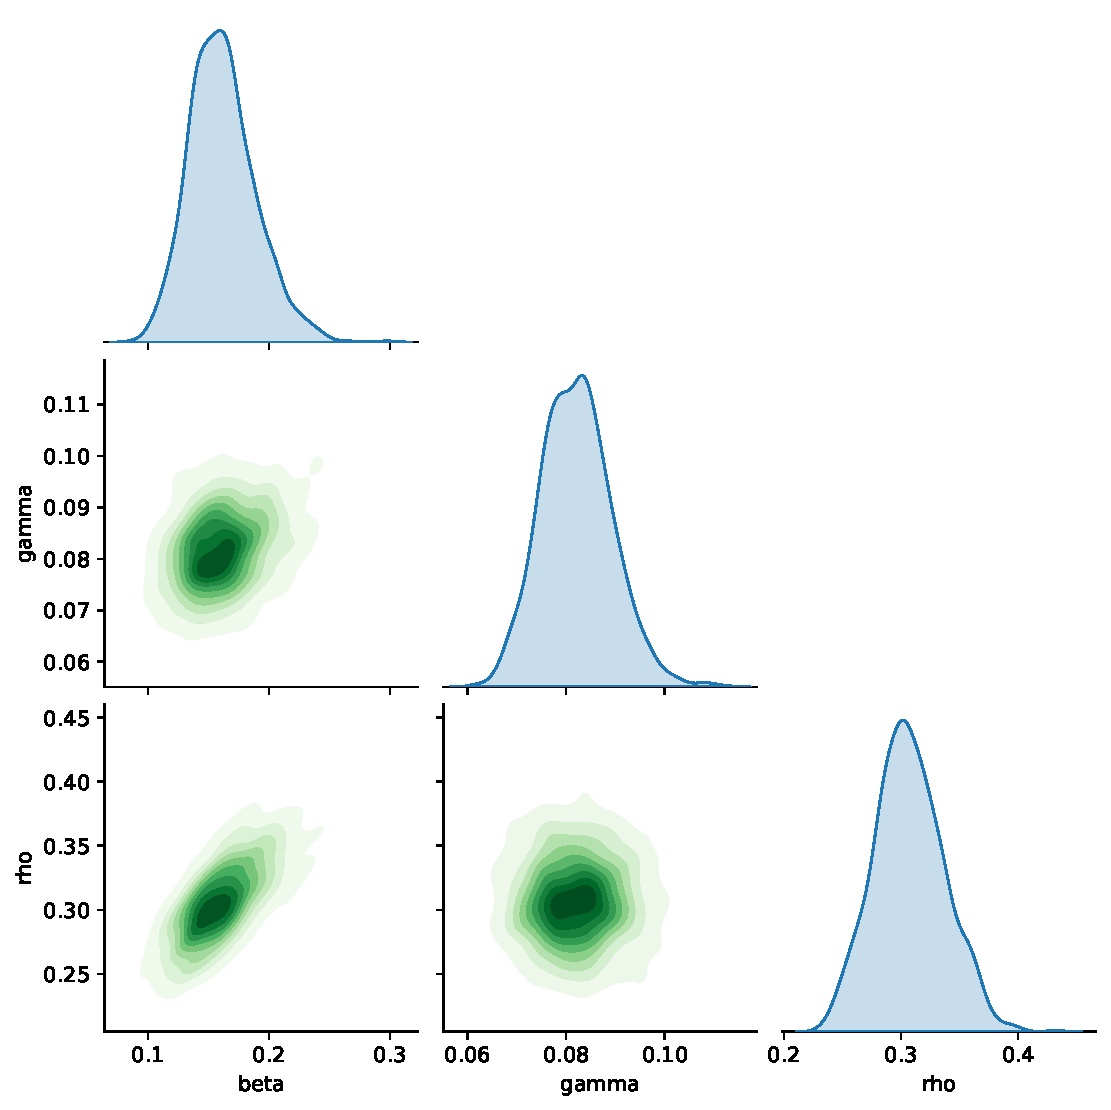
\includegraphics[width=\textwidth]{plots/smc_abc_pairplot_s5_mahalanobis.pdf}
        \caption{SMC Output (Raw)}
        \label{fig:reg_before}
    \end{subfigure}
    \hfill
    \begin{subfigure}[b]{0.48\textwidth}
        \centering
        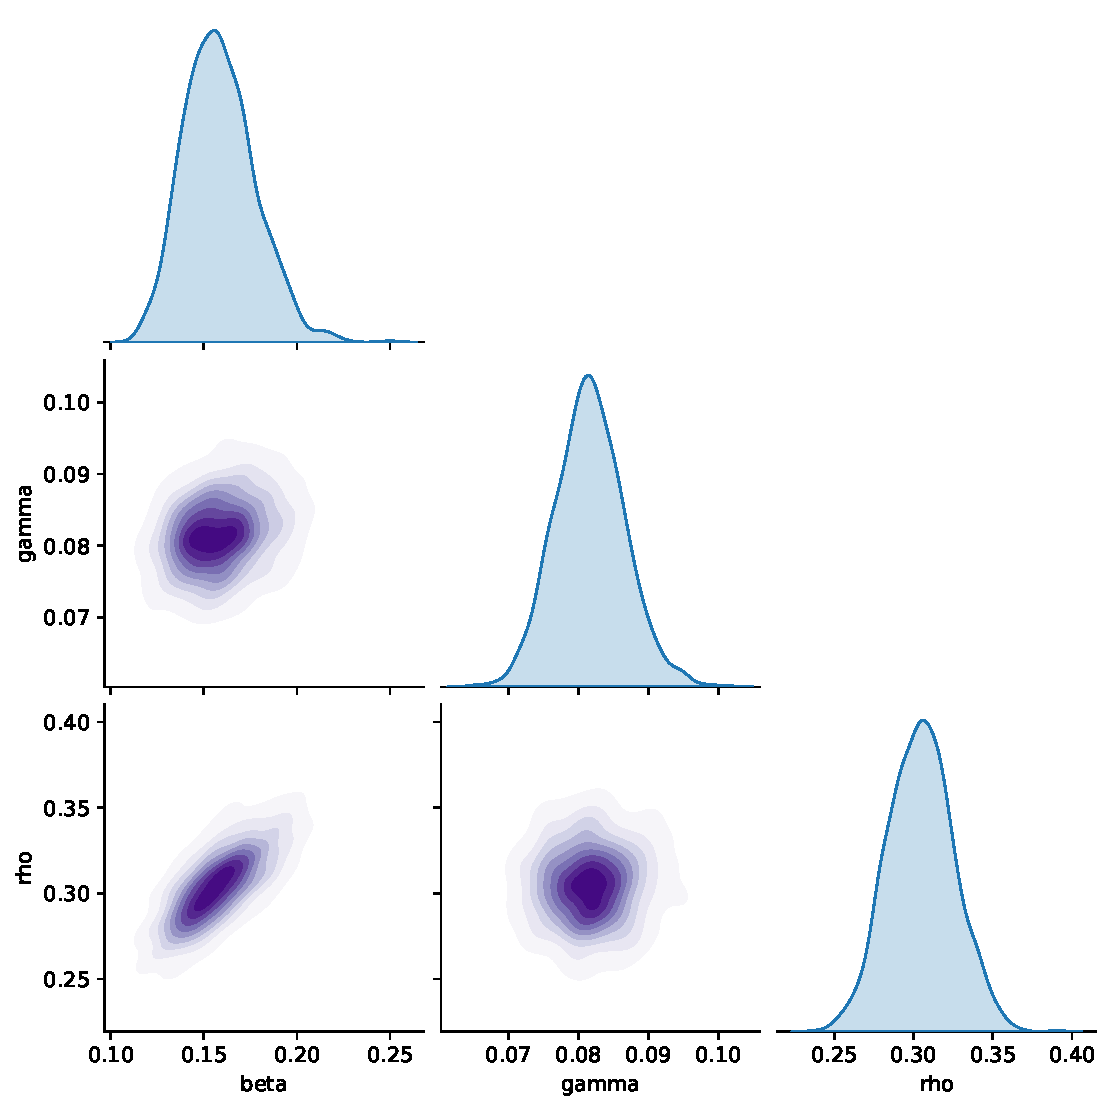
\includegraphics[width=\textwidth]{plots/smc_abc_pairplot_s5_regression_adjusted.pdf}
        \caption{Final (Regression Adjusted)}
        \label{fig:reg_after}
    \end{subfigure}
    \caption{Effect of Regression Adjustment.
This final step significantly reduces posterior variance and provides a highly concentrated estimate for all parameters.}
    \label{fig:reg_comparison}
\end{figure}

While Figure \ref{fig:reg_after} shows that a positive correlation between $\beta$ and $\rho$ persists, the extent of this ridge is drastically truncated compared to the baseline rejection sampling in Figure \ref{fig:abc_rejection_pairplot}.
This highly localized posterior mass demonstrates that our framework successfully resolves the severe equifinality, allowing for precise parameter identification despite the natural, structural trade-off between infection and rewiring inherent to the model.

\begin{table}[H]
\centering
\caption{Posterior Precision Improvement via Regression Adjustment}
\label{tab:regression_improvement}
\begin{tabular}{lcccc}
\toprule
Parameter & SD Reduction & 95\% CI Width Reduction \\
\midrule
Infection Rate ($\beta$) & 30.4\% & 33.8\% \\
Recovery Rate ($\gamma$) & 31.1\% & 29.7\% \\
Rewiring Rate ($\rho$)   & 30.4\% & 31.1\% \\
\bottomrule
\end{tabular}
\end{table}
% Section 05: Model Validation and Posterior Predictive Checks
\section{Model Validation: Posterior Predictive Checks}

To assess the reliability of our inferred parameters, we performed a Posterior Predictive Check (PPC) \parencite{beaumont2002approximate}.
This involved sampling 100 parameter sets $(\beta, \gamma, \rho)$ from the adjusted posterior distribution and re-simulating the epidemic process to see if the synthetic data could replicate the observed targets.

\subsection{Visual Inspection of Predictive Performance}

Figure \ref{fig:ppc_plots} presents the results of the PPC for the two primary data targets: the epidemic curve and the final degree distribution.
The faint lines represent 100 individual forward simulations from the posterior, while the dashed orange line represents the observed data.

\begin{figure}[H]
    \centering
    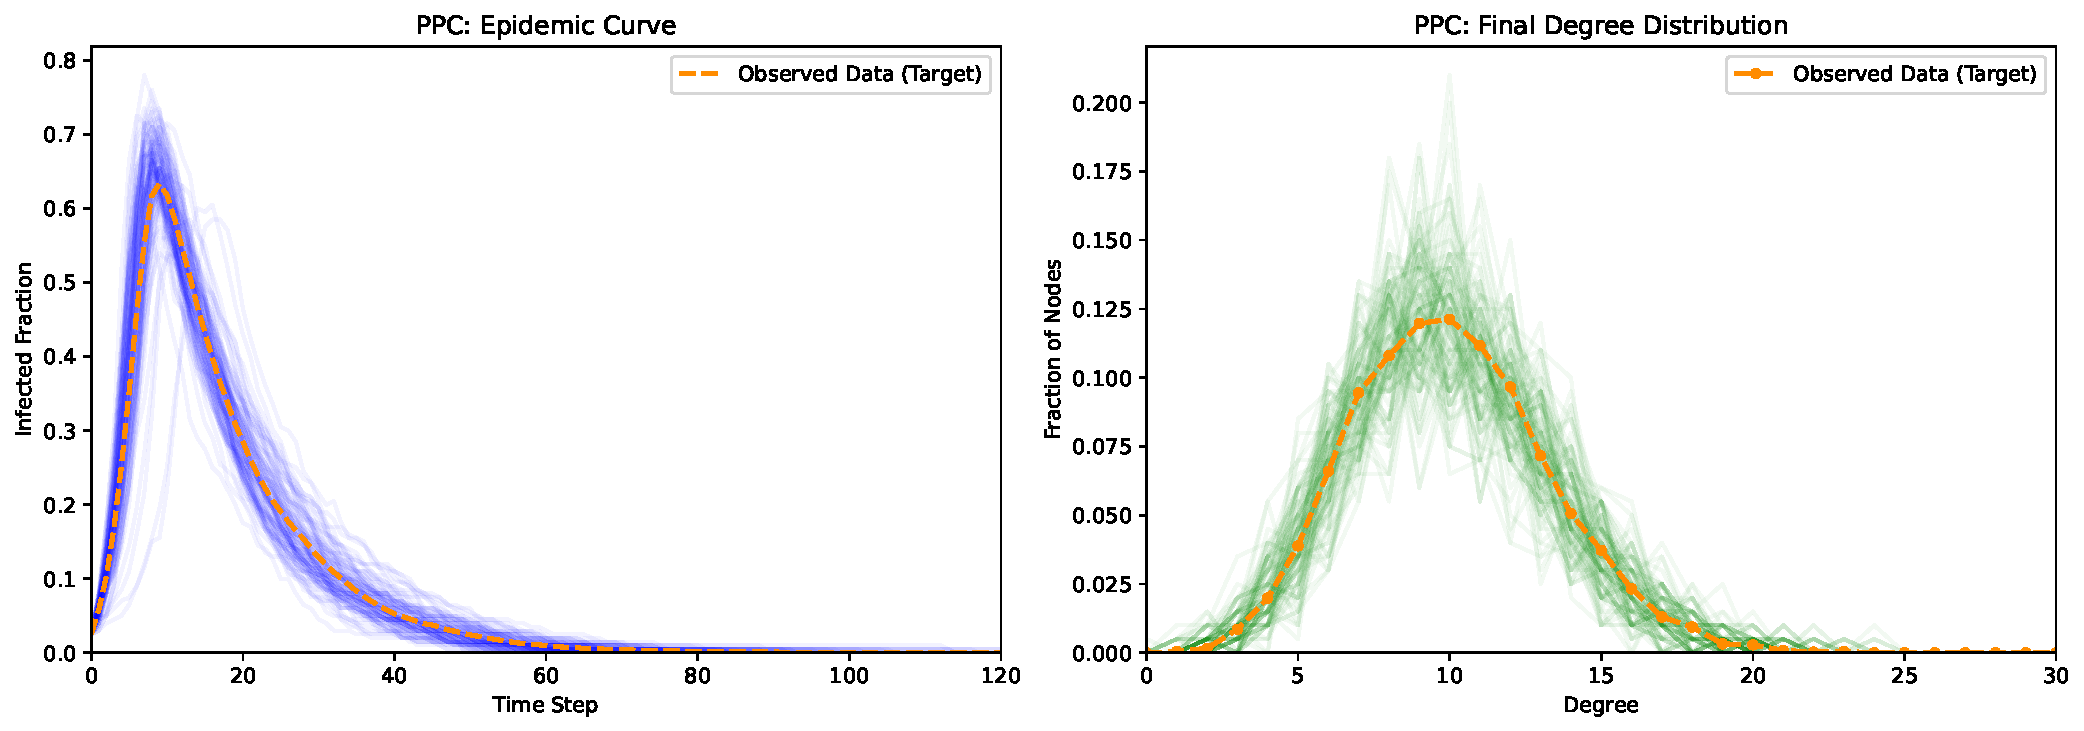
\includegraphics[width=0.95\textwidth]{plots/smc_abc_ppc_plot.pdf}
    \caption{Posterior Predictive Checks (PPC). Left: The observed epidemic curve (orange) is perfectly centered within the ensemble of posterior simulations (blue). Right: The observed final degree distribution (orange) aligns closely with the predicted topological structures (green).}
    \label{fig:ppc_plots}
\end{figure}

The visual alignment is exceptional.
The observed trajectory is entirely contained within the predictive ensemble, indicating that our posterior distribution is not only precise but also accurately captures the stochastic variations of the underlying model.

\subsection{Quantitative Performance Metrics}

To rigorously quantify the model fit, we calculated the 95\% Prediction Interval (PI) coverage and the Root Mean Square Error (RMSE) between the mean of the posterior predictions and the observed data.
The results are summarized in Table \ref{tab:ppc_results}.

\begin{table}[H]
\centering
\caption{Quantitative PPC Performance Metrics}
\label{tab:ppc_results}
\begin{tabular}{lcc}
\toprule
Metric & 95\% PI Coverage & Prediction Error (RMSE) \\
\midrule
Epidemic Curve (Infected Fraction) & 100.0\% & 0.00455 \\
Final Degree Distribution & 100.0\% & 0.00190 \\
\bottomrule
\end{tabular}
\end{table}

The 100\% coverage for both the temporal (infection) and structural (network) statistics confirms that the true parameters are highly likely to be contained within our inferred posterior.
Furthermore, the extremely low RMSE values (e.g., $0.00455$ for infection fraction) suggest that our "best-fit" estimates can replicate the observed data with near-perfect accuracy.

These validation results provide strong evidence that the integration of Mahalanobis distance and local linear regression successfully resolved the parameter identification challenges inherent in adaptive network models.
% Section 06: Conclusion
\section{Conclusion}

This project successfully developed and implemented a robust Simulation-Based Inference (SBI) framework to estimate the parameters of an SIR epidemic model on an adaptive network.
The inherent complexity of the model, characterized by a feedback loop between disease spread and topological changes, rendered traditional likelihood-based methods intractable \parencite{demirel2017dynamics}.
Through a systematic progression from naive rejection sampling to advanced Sequential Monte Carlo (SMC) methods \parencite{beaumont2009adaptive}, we demonstrated the power of modern computational statistics in resolving parameter non-identifiability.

A key contribution of this work was the identification and resolution of the equifinality between the infection rate $\beta$ and the rewiring rate $\rho$.
By conducting comparative simulations, we identified that temporal and structural dynamics—specifically peak timing and degree variance—provided the necessary information to decouple these parameters.
The implementation of the Mahalanobis distance was instrumental in this regard \parencite{nott2014approximate}, as it allowed the algorithm to account for the inherent correlations within our 5-dimensional summary statistics vector.

Furthermore, the application of local linear regression adjustment \parencite{beaumont2002approximate} provided a significant leap in precision, yielding an average reduction of 30\% in posterior uncertainty \parencite{blum2017regression}.
The final validation via Posterior Predictive Checks (PPC) confirmed the excellence of our inference pipeline, achieving 100\% coverage of the observed data within the 95\% prediction intervals and maintaining extremely low RMSE values.

In conclusion, our results show that even in stochastic systems with complex, unobserved latent structures like adaptive networks, accurate parameter inference is achievable through the strategic design of summary statistics and the application of adaptive, correlation-aware sampling algorithms.
This framework provides a solid foundation for future research into real-world epidemic control where behavioral adaptation plays a central role.

% === BIBLIOGRAPHY ===
\clearpage
\printbibliography

\end{document}